\chapter{Natural User Interfaces}
\textit{“Until now, we have always had to adapt to the limits of technology and conform
the way we work with computers to a set of arbitrary conventions and procedures.
With NUI, computing devices will adapt to our needs and preferences for the first
time and humans will begin to use technology in whatever way is most
comfortable and natural for us.”} 

[Bill Gates, co-founder of Microsoft]
\\
\\Le NUI puntano ad invertire il paradigma di interazione classico: sono il livello massimo della progettazione antropocentrica. Sono interfacce \textbf{naturali e facili da usare, la cui interazione con l'utente è diretta, intuitiva e basata su movimenti assoluti}. \\
Al contrario di ciò che si potrebbe pensare, è stata Microsoft ad investire sullo sviluppo delle Natural User Interfaces (per poi farsi scavalcare da Apple, la quale ora fa da padrona nel mondo delle NUI).


\textbf{Le NUI puntano ad un'eseperienza basata su un comportamento naturale.}
Un comando scritto nella forma "\code{dir /Documents}" non è di tipo naturale. Per avere un'idea di cosa si intenda per comportamento naturale basti pensare all'interazione cliente-fruttivendolo: non verrebbe mai in mente a nessun cliente di comunicare dicendo "list -frutti -verdure". 


Un'interfaccia naturale tipicamente è \textbf{invisibile}, e l'obiettivo del progettista è quello di \textbf{far sparire l'interfaccia}. Esempi di interfacce invisibili sono: 
\begin{itemize}
\item lo schermo di uno smartphone, dove lo schermo è sia un mezzo per l'input che per l'output
\item strumenti di supporto vocale (Amazon Echo, Google Home) dove sono presenti sia microfono che speaker che unità di calcolo.
\item smartwatch con lettore dei battiti cardiaci
\end{itemize}

Sono strumenti che risultano tutt'uno con cui interagire, l'utente non percepisce il distacco funzionale.
É bene sottolineare che naturale non vuol dire biologoico o derivante dalla natura, si intende principalmente che non richiede apprendimento.
\\
\\Le Natural User Interfaces consentono di essere utilizzate facendo leva sull'esperienza di interazione col mondo naturale dell'utilizzatore. Il modello concettuale, le affordances e i significanti sono correlabili con quelli del mondo reale, ciò riduce notevolemnte (se non del tutto) il bisogno di apprendere per utilizzare queste interfacce.

La transizione tra utente novizio ed esperto risulta veloce dato che il modello concettuale è comprensibile in fretta e il processo di apprendimento (dove presente) è quasi istantaneo.
\\
\\Nella pratica è pressochè impossibile realizzare un'interfaccia che richieda zero apprendimento.\\
In una NUI dobbiamo far sì che l'utente sia sin da subito in grado di usare le funzioni base. Dev'essere poi l'interfaccia stessa a guidare l'utente verso funzioni avanzate.

Si può pensare alla NUI e al relativo processo di apprendimento come la relazione che si instaura con un cane o con un figlio appena nato: una persona sa come interagire basilarmente con un cane o un neonato ma è solo tramite l'esperienza che imparerà a consoscere le motivazioni dei loro comportamenti e quindi a capire come comportarsi di conseguenza. Domande che inizialmente potrebbero sorgere sono: \textit{da dove deve essere inserito il cibo? dov'è il libro di manutenzione del bambino?}
\\
\\"Naturale" fa riferimeno al tipo di UX che quell'interfaccia é in grado di abilitare, fa riferimento al \textbf{goal della UX} (ricordando che si può solamente progettare \textbf{per} la UX).
Se si decide di progettare un'interfaccia naturale allora si sta progettando un sistema che va a creare con l'utente un'interazione naturale, basata sulla sua conoscenza esistente.\\
Proprio per questo possono sorgere dei problemi: non tutti gli utenti sono uguali e le differenze culturali incidono sulla progettazione delle interfacce, a causa delle diverse interpretazioni di vincoli e simboli.\\

\section{Limiti delle NUI}
\begin{itemize}
\item \textbf{non tutto è realizzabile tramite NUI}. 
\item la \textbf{complessità} delle funzioni abilitate deve essere \textbf{bassa}
\item \textbf{nessuna interfaccia utente può essere naturale in tutti i contesti  e per tutti gli utenti}
\end{itemize}
I primi due punti derivano dalla necessità di creare interfacce intuitive. Se non si può chiedere all'utente di "studiare" per sostenere l'interazione ci si trova obbligati a non poter oltrepassare una certa soglia di complessità. Si vuole che il modello concettuale della NUI sia facilmente comprensibile.\\
Un foglio di calcolo elettronico non è naturale, non esiste niente in natura di simile: l'utente è obbligato a "studiare" per avere una buona interazione con esso.\\
Al contrario prendere in mano una foto è un'azione naturale così come ruotarla tenendola per 2 angoli.
Le funzioni implemenbtabili tramite NUI sono \textbf{poche}.\\
\\Poichè le NUI si appoggiano a skill acquisite durante la nostra vita, \textbf{minimizzano il carico cognitivo necessario }per interagire col sistema.\\
Non si può progettare una NUI senza prendere in considerazione il contesto di utilizzo. Può essere utile pensare ad un coltello: il suo uso dipende dal contesto. Un chirurgo può usarne uno in sala operatoria ed uno nella sua cucina per affettare le verdure (non c'è differenza funzionale tra un coltello e un bisturi). \\Se si volesse realizzare un'interfaccia grafica per un'app che permette di editare foto si deve prendere in considerazione la differenza fra un casual user ed un professionista.
\textbf{Nessuna interfaccia utente può essere naturale in tutti i contesti  e per tutti gli utenti.}\\
È importante ricordare che ciò che è NUI per un utente non è detto lo sia per un altro. Le NUI sono percepite come intuitive solo se le skill dell'utente in quel contesto sono adeguate a quelle richieste dall'interfaccia.
Si può avere \textbf{instant learning }solo se si possiede il bagaglio culturale necessario per apprendere interagendo.\\
(Non vanno bene per tutte le stagioni!)\\

\section{Come si arriva alle NUI?}
\begin{figure}[!h]
	\centering
	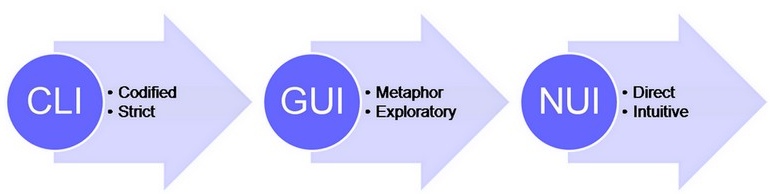
\includegraphics[scale=0.4]{immagini/CLItoNUI.png}
	\caption{}
\end{figure}
Analizzando le CLI (Command Line Interface) ci si può accorgere che esse sono quasi l'opposto delle NUI: sono codificate, fortemente vincolate e seguono una sintassi precisa con comandi predefiniti.
La conoscenza richiesta é \textbf{enorme}, inizialmente non si è neanche in grado di digitare il comand \code{help} se si è totalmente a digiuno di interazioni di tipo CLI.
\\
\\Passando alle GUI si può dire che sono basate su:
\begin{itemize}
\item metafore
\item modalità esplorativa
\end{itemize}

\textbf{Tramite la metafora si apprende esplorando}. Si scopre ad esempio che le cartelle contengono file, che con un click si può porre l'attenzione su un file mentre con 2 click lo si può aprire. Anche il cestino è una metafora: vi si inserisce ciò che non serve più e finchè non si "svuota" il sacchetto rimane pieno.
\\
\\Le NUI sono invece dirette e intuitive. L'intuito è importante in questo contesto: ci fa sentire confidenti, come se ciò che si deve fare per la prima volta lo si fosse già fatto.\\
Ad esempio l'interazione basilare con un tablet è intuitiva: la nostra mano è attratta dal toccare le icone, si scopre così che sono cliccabili. Ma non si capisce subito che si possono spostare ad esempio, questa è una funzione avanzata e dovrà essere proprio l'interfaccia a veicolarlo successivamente.
\\
\\ Vi è qui un cambio di paradigma rispetto al pensiero comune dell'informatico per cui tutte le funzioni sono importanti allo stesso modo.\\
Molte funzioni vengono così scoperte per caso, sbagliando. Gli errori diventano un allenamento per imparare nuove funzioni: è proprio questo il processo di apprendimento continuo che si ha nelle NUI.\\
É bene progettare le NUI per far sì che le azioni siano del tutto simili a quelle che si avrebbero con il corrispondente oggeto reale: il mondo digitale diviene metafora per quello reale.\\
Le seguenti caratteristiche sono utili per capire cosa NON è una NUI.\\
\\
\textit{“Voice, gesture, touch does not necessarily Natural User Interface make.”}

[Bill Buxton, Principal Researcher at Microsoft]
\\
\\Si può avere una NUI con o senza la funzione di speech. Può essere utile averla ma non è una condizione nè necessaria nè sufficiente.\\
Con un touchpad non si può avere una NUI, poichè l'interazione non è diretta .\\
\\Sono state individuate da Joshua Blake \textbf{4 linee guida}:
\begin{itemize}
\item Instant expertise
\item Progressive learning
\item Direct Interaction
\item Low cognitive load
\end{itemize}

\textbf{L'obiettivo del design è soddisfare i bisogni dell'utente, non dover insegnare qualcosa agli utenti}.


\section{Reality Based Interface}
Per Reality-based Interface si intende un modello di interazione che esiste nella realtà e che viene virtualizzato. \\
Possono essere RBI sia la realtà virtuale (es: Oculus Rift) che la realtà aumentata (augmented, es: Pokémon Go oppure cliccare su una lattina reale e avere delle informazioni aggiuntive).\\
\textbf{Fare una NUI non implica che si sta realizzando una RBI, mentre fare una RBI solitamente implica realizzare una NUI}.\\
\begin{figure}[!h]
	\centering
	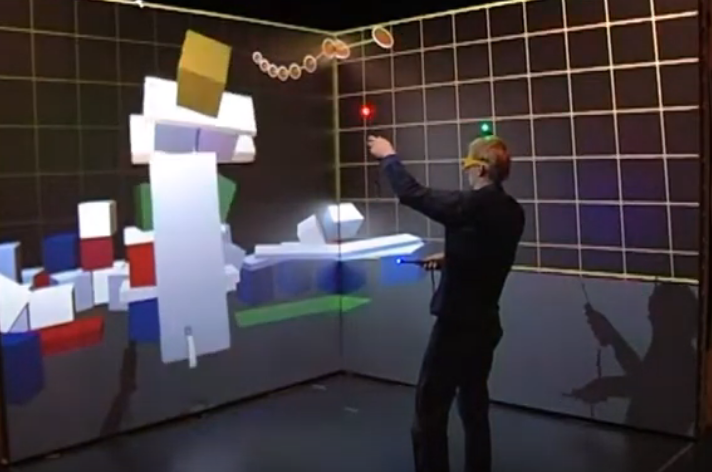
\includegraphics[scale=0.4]{immagini/ruis.png}
	\caption{RUIS: Reality-based User Interface System}
\end{figure}
\\NUI e RBI sono quindi diverse, ciò che le accomuna maggiormente è che l'utente non deve far altro che basarsi sulle proprie esperienze pregresse per interagire.\\
Se si virtualizza il mondo reale anche il mondo virtuale risultante si baserà sugli stessi paradigmi d'interfacciamento.\\

\pagebreak

